% 2011 年四川卷理科第 15 题：半径为 R 的球 O 的内接圆柱（侧面积最大时）。
% 来源 PDF：普通高考/2011/2011四川理.pdf，SHA-256 116ce515679869425079ef4777505df3735ba4cba64847c9069b7d7acdb4fda4。
% 原页：第 1 页（A3 三栏）第 2 栏下部，书页码 701。
% 重绘依据：照原页——外轮廓为球的大圆；圆柱上下底画成扁椭圆，
%   上底整圈实线（俯视可见），下底前半实线、后半虚线；圆柱两条母线为虚线；
%   球的赤道前半实线、后半虚线；O 为球心（实心点），R 由 O 连到上底圆周上一点（虚线）。
% 比例取 r=0.73R、高=0.68R（r^2+(h/2)^2=R^2），与原页大致相符，不严格按比例。
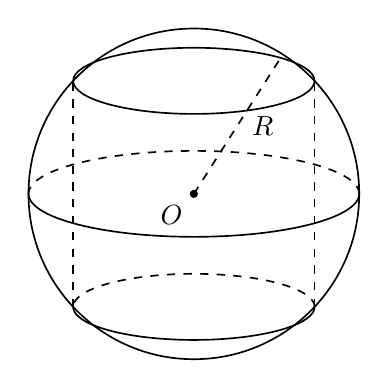
\begin{tikzpicture}[scale=1.05, >=stealth, semithick]
  % 球的大圆
  \draw (0,0) circle (2);

  % 球的赤道：前半实线，后半虚线
  \draw[domain=180:360, samples=60] plot ({2*cos(\x)},{0.52*sin(\x)});
  \draw[dashed, domain=0:180, samples=60] plot ({2*cos(\x)},{0.52*sin(\x)});

  % 圆柱上底（整圈可见）
  \draw (0,1.367) ellipse ({1.46} and {0.40});

  % 圆柱下底：前半实线，后半虚线
  \draw[domain=180:360, samples=60] plot ({1.46*cos(\x)},{-1.367+0.40*sin(\x)});
  \draw[dashed, domain=0:180, samples=60] plot ({1.46*cos(\x)},{-1.367+0.40*sin(\x)});

  % 圆柱母线（原页为虚线）
  \draw[dashed] (-1.46,-1.367) -- (-1.46,1.367);
  \draw[dashed] (1.46,-1.367) -- (1.46,1.367);

  % 球心与半径
  \fill (0,0) circle (1.4pt);
  \node[below left, inner sep=2pt] at (-0.06,-0.06) {$O$};
  \draw[dashed] (0,0) -- (1.05,1.645);
  \node[below right, inner sep=1pt] at (0.66,0.98) {$R$};
\end{tikzpicture}
